%%%%%%%%%%%%%%%%%%%%%%%%%%%%%%%%%%%%%%%%%
% Short Sectioned Assignment LaTeX Template Version 1.0 (5/5/12)
% This template has been downloaded from: http://www.LaTeXTemplates.com
% Original author:  Frits Wenneker (http://www.howtotex.com)
% License: CC BY-NC-SA 3.0 (http://creativecommons.org/licenses/by-nc-sa/3.0/)
%%%%%%%%%%%%%%%%%%%%%%%%%%%%%%%%%%%%%%%%%

%----------------------------------------------------------------------------------------
%	PACKAGES AND OTHER DOCUMENT CONFIGURATIONS
%----------------------------------------------------------------------------------------

\documentclass[paper=a4, fontsize=11pt]{scrartcl} % A4 paper and 11pt font size

% ---- Entrada y salida de texto -----

\usepackage[T1]{fontenc} % Use 8-bit encoding that has 256 glyphs
\usepackage[utf8]{inputenc}
%\usepackage{fourier} % Use the Adobe Utopia font for the document - comment this line to return to the LaTeX default

% ---- Idioma --------

\usepackage[spanish, es-tabla]{babel} % Selecciona el español para palabras introducidas automáticamente, p.ej. "septiembre" en la fecha y especifica que se use la palabra Tabla en vez de Cuadro

% ---- Otros paquetes ----

\usepackage{url} % ,href} %para incluir URLs e hipervínculos dentro del texto (aunque hay que instalar href)
\usepackage{amsmath,amsfonts,amsthm} % Math packages
%\usepackage{graphics,graphicx, floatrow} %para incluir imágenes y notas en las imágenes
\usepackage{graphics,graphicx, float} %para incluir imágenes y colocarlas

\usepackage{listings}	%para incluir remarcado para comandos bash

% Para hacer tablas comlejas
%\usepackage{multirow}
%\usepackage{threeparttable}

%\usepackage{sectsty} % Allows customizing section commands
%\allsectionsfont{\centering \normalfont\scshape} % Make all sections centered, the default font and small caps

\usepackage{fancyhdr} % Custom headers and footers
\pagestyle{fancyplain} % Makes all pages in the document conform to the custom headers and footers
\fancyhead{} % No page header - if you want one, create it in the same way as the footers below
\fancyfoot[L]{} % Empty left footer
\fancyfoot[C]{} % Empty center footer
\fancyfoot[R]{\thepage} % Page numbering for right footer
\renewcommand{\headrulewidth}{0pt} % Remove header underlines
\renewcommand{\footrulewidth}{0pt} % Remove footer underlines
\setlength{\headheight}{13.6pt} % Customize the height of the header

\numberwithin{equation}{section} % Number equations within sections (i.e. 1.1, 1.2, 2.1, 2.2 instead of 1, 2, 3, 4)
\numberwithin{figure}{section} % Number figures within sections (i.e. 1.1, 1.2, 2.1, 2.2 instead of 1, 2, 3, 4)
\numberwithin{table}{section} % Number tables within sections (i.e. 1.1, 1.2, 2.1, 2.2 instead of 1, 2, 3, 4)

\setlength\parindent{0pt} % Removes all indentation from paragraphs - comment this line for an assignment with lots of text

\newcommand{\horrule}[1]{\rule{\linewidth}{#1}} % Create horizontal rule command with 1 argument of height

\usepackage{booktabs}
\usepackage{tabularx}
\usepackage{multicol} 

%----------------------------------------------------------------------------------------
%	TÍTULO Y DATOS DEL ALUMNO
%----------------------------------------------------------------------------------------

\title{
\normalfont \normalsize 
\textsc{\textbf{Ingeniería del conocimiento (2020-2021)} \\ Máster en ingeniería informática \\ Universidad de Granada} \\ [25pt] % Your university, school and/or department name(s)
\horrule{0.5pt} \\[0.4cm] % Thin top horizontal rule
\huge Práctica de redes neuronales \\ % The assignment title
\horrule{2pt} \\[0.5cm] % Thick bottom horizontal rule
}
\author{Manuel Orantes Taboada} % Nombre y apellidos

\date{\normalsize\today} % Incluye la fecha actual

%----------------------------------------------------------------------------------------
% DOCUMENTO
%----------------------------------------------------------------------------------------

\begin{document}

\maketitle % Muestra el Título

\newpage %inserta un salto de página

\tableofcontents % para generar el índice de contenidos

\newpage

\section{Introducción}

La base de datos MNIST está formada por muchas imágenes de números manuscritos. En ella podemos apreciar las imágenes con tamaño 32x32 píxeles en escalas de blancos y negros, en las cuales cada píxel alcanza un valor entre 0 y 255. Tenemos 60000 imágenes en el conjunto train y otras 10000 en el conjunto test. Además, cada imagen tiene asociada una etiqueta con su número correspondiente. El objetivo es realizar un clasificador de números a través de redes neuronales artificiales que sea capaz de clasificar de forma aceptable las imágenes de test, habiendo sido entrenado previamente con las imágenes del conjunto train. 

Para ello, veremos primero una red neuronal multicapa y después varios modelos de redes neuronales convolucionales, que son mucho mejores y conseguirán un mejor resultado. No hemos realizado experimentos de redes neuronales simples ya que, sabemos, que no van a tener un resultado mejor del que podemos obtener con las otras, y queremos obtener el mejor clasificador posible.

Hay que decir que todos los experimentos se han realizado en colab de google.

\section{Primer contacto, tutorial}

En primer lugar, elegí hacer la práctica en python, usando la librería de keras. A modo introductorio de esta librería, usé el tutorial que viene en la propia documentación, en la página \url{https://keras.io/examples/vision/mnist_convnet/}. Como podemos observar, nos encontramos con una red neuronal convolucional, aplicada ya sobre el problema que queremos, MNIST. Indagando un poco más, vemos que se aplicado dos convoluciones, con sus respectivas reducciones mediante la función del máximo, la que suele ser la más usada por sus resultados y por rapidez. A parte de esto, vemos que no tiene ninguna capa interna, solo una capa que cambia el tipo de array y otra que elimina los datos por debajo del umbral 0.5. Por último, está la capa que clasifica usando la función softmax, que siempre suele dar muy buenos resultados. A continuación podemos ver la estructura que actualmente hemos descrito:

\begin{figure}[H]
	\centering
	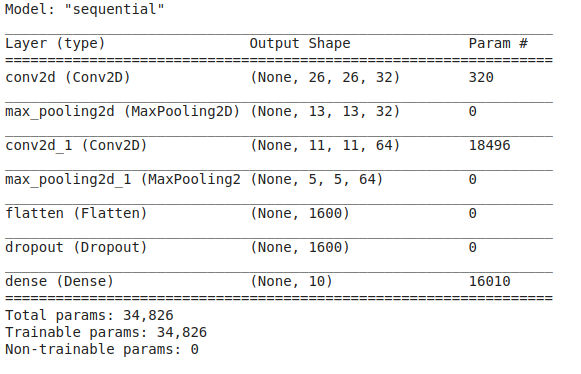
\includegraphics[width=0.55\linewidth]{tutorial}
	\label{fig:tutorial}
\end{figure}

Lo único que añadimos al código que nos ofrece el tutorial es una función para controlar el tiempo y después otra para la salida, que nos da los datos necesarios, error en test y train y el conjunto de etiquetas de salida, en el orden en el que lo obtuvimos.

En este caso, los resultados obtenidos son los siguientes:
\\\\
Error sobre el conjunto de prueba: 0.8199989795684814

Error sobre el conjunto de entrenamiento: 0.33333301544189453

Tiempo de entrenamiento: 983.52
\\\\
Vemos que no está nada mal el resultado, pero, ¿podremos mejorar al tutorial? Al fin y al cabo, la red neuronal no tiene ninguna capa oculta, no puede ser la mejor, ¿no?

\section{Red multicapa}

Aunque seguramente sea peor que la red convolucional, he querido que al menos tengamos una muestra de este tipo de red neuronal. Al fin y al cabo, lo que si vamos a ganar es en el tiempo de entrenamiento, ya que el entrenamiento en este caso va a ser muy rápido, en comparación con las redes convolucionales.

Veamos en primer lugar la estructura de la red neuronal multicapa seleccionada:

\begin{figure}[H]
	\centering
	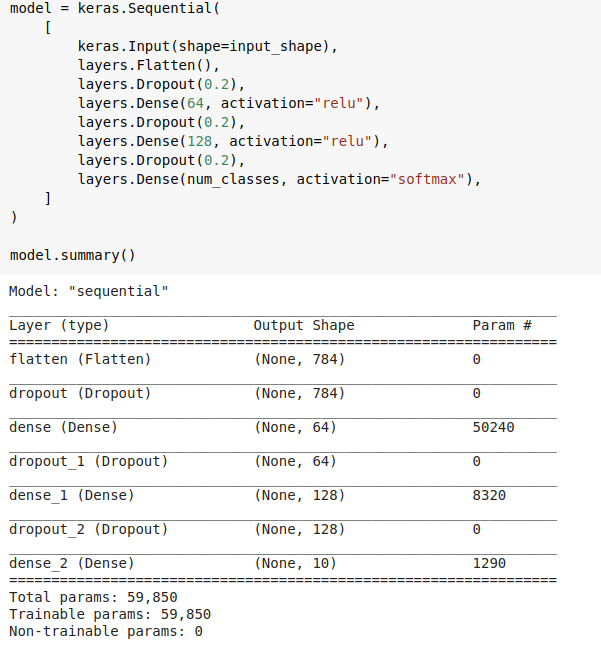
\includegraphics[width=0.7\linewidth]{multicapa}
	\label{fig:multicapa}
\end{figure}

Como podemos ver hemos creado una red con dos capas ocultas, con 64 y 128 neuronas respectivamente de tipo Relu. Además, le añadimos unos dropout para aligerar la red. Veamos los resultados de esta red neuronal:
\\\\
Error sobre el conjunto de prueba: 2.0200014114379883

Error sobre el conjunto de entrenamiento: 1.0633349418640137

Tiempo de entrenamiento: 45.79
\\\\

Como podemos ver, en menos de un minutos tenemos entrenada la red, que alcanza un éxito cercano al 98\%, algo que no está nada mal, al tratarse de una red neuronal que no es convolucional.

\section{Tratamiento de los datos}

Para la siguiente prueba he querido aplicar las técnicas que usé en el curso de Aprendizaje Automático de hace un par de años, del doble grado en ingeniería informática y matemática. Para ello, he querido tratar los datos, por lo que primero he quitado los píxeles que menos repercusión tienen en la imagen. Para ello aplicamos un filtro del siguiente estilo:

sel = VarianceThreshold(threshold=(0.01))
sel.fit\_transform(x\_train)

Y a continuación podemos ver cuales son los píxeles que hemos quitado, en negro:

\begin{figure}[H]
	\centering
	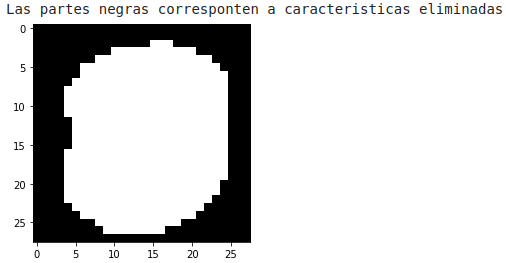
\includegraphics[width=0.7\linewidth]{caracteristicas_eliminadas}
	\label{fig:caracteristicaseliminadas}
\end{figure}

Ahora, la diferencia que tenemos con los otros casos para aplicar las capas a la red neuronal, es que las convoluciones hay que hacerlas en 1D en vez de en 2D. Esta sería la red que hemos montado para este caso:

\begin{figure}[H]
	\centering
	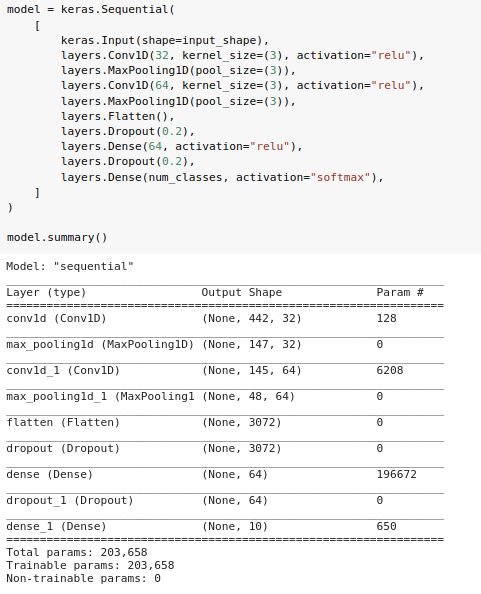
\includegraphics[width=0.4\linewidth]{tratamineto-datos}
	\label{fig:tratamineto-datos}
\end{figure}

Podemos ver los resultados obtenidos:

Error sobre el conjunto de prueba: 1.8499970436096191

Error sobre el conjunto de entrenamiento: 0.3166675567626953

Tiempo de entrenamiento: 587.77
\\\\

Vemos que mejora a la red multicapa, pero basta a la vista que no hemos mejorado nada con respecto a la convolucional del tutorial, por lo que, esta decisión, parece no aportar ninguna mejora, y será descartada.

\section{Siguientes experimentos}

A partir de este experimento, hemos hecho muchos experimentos, aunque muchos de ellos no han sido enviados por el formulario de google. En estos experimentos se ha probado:

\subsection{Número de epoch}

Se han probado desde pocas épocas (10-15) hasta muchas (75-100) y al final, los resultados al final muestran que, aunque se mejora el modelos para train, para test no pasa lo mismo,debido quizás al sobre entrenamiento, y por lo tanto al final se ha decidido que los mejores resultados en distintos experimentos han sido en torno a 20-25 épocas, y estos números son los que se usarán.

\subsection{batch\_size}

Se han probado distintos tamaños, 64, 128, 256... Al final, a base de probar se ha decidido que los mejores resultados se obtienen con 128.

\subsection{Algoritmo de entrenamiento}
No se han probado muchos, pero adam es un algoritmo bastante consistente y ha sido el seleccionado para las distintas pruebas que se han realizado.

\subsection{Tipo de neuronas}
Se han probado muchos de los tipos que encontramos en la documentación oficial \url{https://keras.io/api/layers/activations/} y por lo general, los que mejores resultados han dado son los de tipo relu, aunque a veces se obtienen buenos resultados mezclando estos tipos de capas con otras de neuronas de tipo Elu y Selu.

\subsection{Mascaras de convolución}
Se han intentado con dos mascaras, con una y con tres. Los resultados son demoledores al hecho de usar dos máscaras solamente.

A continuación vamos a mostrar los datos de algunos de los experimentos con sus resultados, aunque, como bien hemos dicho antes, no todos los experimentos han sido enviados por el formulario de google (todas las red convolucionales tienen la misma convolución 2D, de 64 y 128 neuronas tipo relu con MaxPooling entre cada una y además la misma salida usando softmax):
\\\\
Red convolucional con dos capas ocultas de 64 y 128 neuronas tipo Relu

Error sobre el conjunto de prueba: 0.5900025367736816

Error sobre el conjunto de entrenamiento: 0.3016650676727295

Tiempo de entrenamiento: 702.65
\\\\

Red convolucional con dos capas de 128 y 64 neuronas tipo Relu (en ese orden)

Error sobre el conjunto de prueba: 0.6900012493133545

Error sobre el conjunto de entrenamiento: 0.0816643238067627

Tiempo de entrenamiento: 991.64
\\\\

Red convolucional con una capa de 128 neuronas tipo Relu

Error sobre el conjunto de prueba: 0.7300019264221191

Error sobre el conjunto de entrenamiento: 0.10833144187927246

Tiempo de entrenamiento: 899.2
\\\\
\newpage
Red convolucional con dos capas ocultas de 64 y 128 neuronas tipo Selu

Error sobre el conjunto de prueba: 0.6200015544891357

Error sobre el conjunto de entrenamiento: 0.2499997615814209

Tiempo de entrenamiento: 1025.02
\\\\

Red convolucional con dos capas ocultas de 64 y 128 neuronas tipo Elu

Error sobre el conjunto de prueba: 0.6699979305267334

Error sobre el conjunto de entrenamiento: 0.18166899681091309

Tiempo de entrenamiento: 1009.33
\\\\
Como podemos ver, aunque a veces el entrenamiento es bastante mejor que en otros, el resultado al aplicar el clasificador al conjunto test no es ni mucho menos el óptimo, por lo que no es necesariamente mejor buscar la excelencia en cuanto al clasificador en el conjunto train.

Se pueden ver los códigos de los experimentos en el Github https://github.com/manuelorantes/IC.

\section{Mejor experimento}

Al final de varias pruebas, vimos que los mejores resultados los obteníamos con capas Relu, después añadimos una tercera capa y mejoró, y lo mismo con la cuarta. Se probó a mezclar capas Elu, Selu y distinto tamaños de dropout y epoch. Al final, el mejor resultado que se consiguió tiene la siguiente estructura:

\begin{figure}[H]
	\centering
	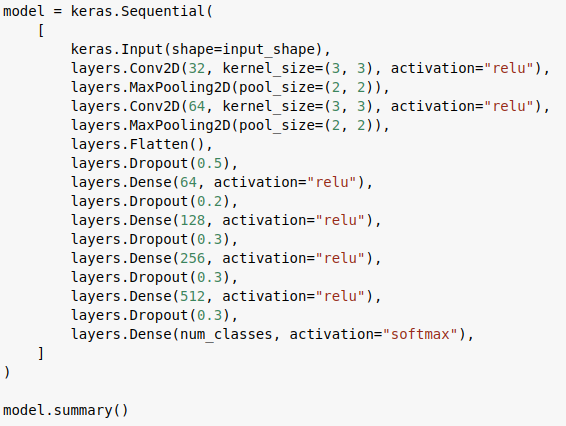
\includegraphics[width=0.7\linewidth]{mejor}
	\label{fig:mejor}
\end{figure}
\newpage
Podemos ver que se ha optado por una red con dos máscaras de convolución relu y sus correspondientes MaxPooling, 4 capas ocultas de 64, 128, 256 y 512 neuronas Relu con Dropout de diferentes pesos. Por último la capa de softmax siempre presente al final de todas nuestras redes.


\section{Conclusiones}
Al final hemos ido realizando distintas pruebas, que en total habrán sido más de 50. Hemos partido de distintos puntos y cuando íbamos encontrando mejores redes hemos ido modificando poco a poco hasta conseguir una mejor. La mayor conclusión que hemos visto es que no basta con aumentar las capas, ni aumentar los epoch ni si quiera acercarse lo máximo posible a los datos del train, ya que pueden provocar sobre entrenamiento.

\end{document}